Ce document présente le travail effectué dans le cadre du projet de deuxième année (PFA) de l'ENSEIRB-MATMECA qui avait pour objectif la création d'un simulateur pour robots.
Il opposera le cahier des charges et les choix de conception au produit finalement obtenu. Cela permettra de mettre en évidence les difficultés rencontrées lors du développement du projet, les choix et concessions qu'il a fallu faire au cours des derniers mois. Chacune de ces difficultés a permis aux membres de l'équipe d'acquérir de nouvelles compétences.

\section{Le contexte}

Le cadre de ce projet de PFA était peu commun puisqu'il a été soumis et réalisé par des élèves de l'école. Il s'agit de l'association de robotique de l'école, EIRBOT. Le sujet a donc été proposé par l'association pour améliorer son potentiel lors de la Coupe de France de robotique. Elle rassemble chaque année près de 200 équipes. De nombreuses équipes s'appuient sur une expérience longue de plusieurs années et utilisent des logiciels de simulation et bibliothèques améliorés d'année en année. Ce projet a donc pour objectif de permettre à Eirbot de fiabiliser ses robots, de faciliter l'écriture du code de stratégie, et ainsi de progresser dans le classement. Néanmoins l'association ne pouvant être cliente du PFA (car représentée par des élèves de deuxième année), l'enseignant chercheur Aymeric Vincent a accepté de tenir le rôle du client.

\begin{figure}[!h]
\centering
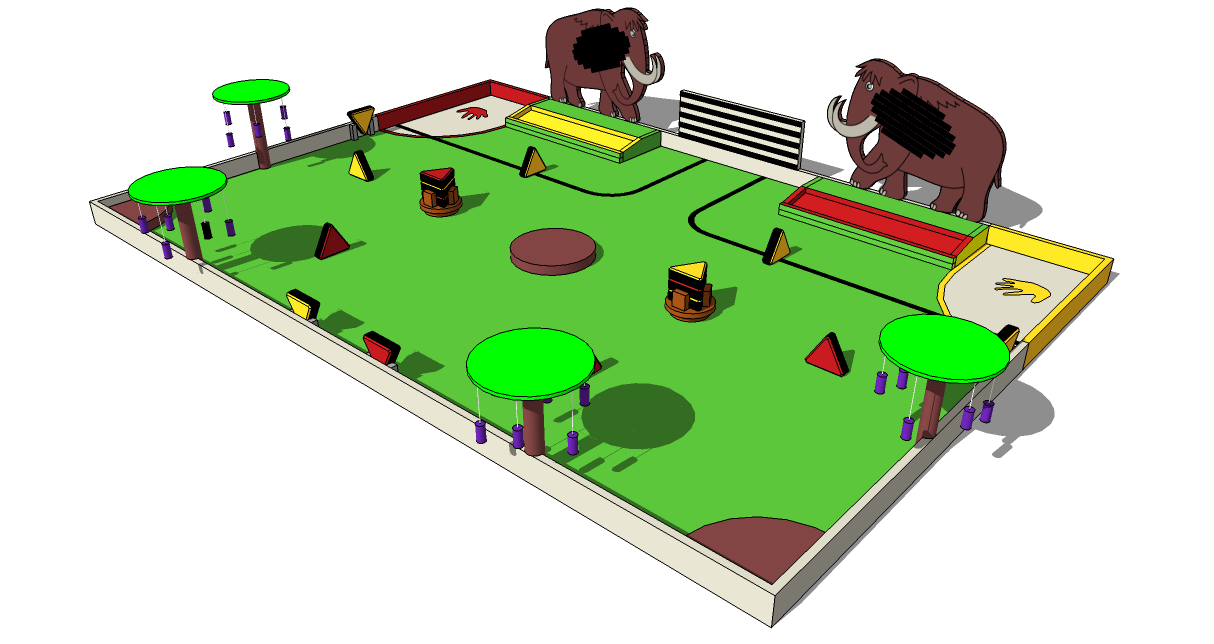
\includegraphics[scale=0.33]{table}
\caption{Table de jeu de l'édition 2014.}
\label{table}
\end{figure}

\paragraph{}
Afin d'avoir une meilleure idée de ce sur quoi s'appuie ce projet, nous proposons une rapide description du règlement de la coupe 2014 et du robot des deuxièmes années.

Comme chaque année, les robots doivent partir d'une zone délimitée de la table. À partir du top départ, ils disposent de 90 secondes pour marquer un maximum de points. Le moyen de faire des points diffère d'année en année. Cette année il est possible de :
\begin{itemize}
\item Récupérer les fruits pendus aux arbres en bord de table pour les verser dans le bac de sa couleur (au pied des mammouths)
\item Faire tomber les triangles, avec la couleur de son équipe face visible
\item Poser une "peinture" de sa couleur sur la fresque entre les deux mammouths
\item Lancer des balles de ping pong sur le velcro des mammouths
\item Lancer un filet au dessus d'un mammouth
\end{itemize}
En plus de marquer des points, le robot doit pouvoir éviter les robots adverses, ou au moins s'arrêter. À la fin des 90 secondes, les robots s'arrêtent et les arbitres procèdent au décompte des points.

\begin{figure}[!h]
\centering

\includegraphics[scale=0.1]{robot}
\caption{Aperçue du robot des deuxièmes années.}
\label{robot}
\end{figure}

\paragraph{}
Le robot n'est pas encore terminé, mais son fonctionnement actuel est quasiment final. Sa stratégie sera basée sur un déplacement précis qui permettra de récupérer les fruits, les mettre dans le bac correspondant, placer les peintures sur la fresque, et lancer les balles sur les mammouths. En fin de match il essaiera de lancer le filet sur un mammouth. Pendant les matchs, il essaiera également de faire tomber des triangles du bon côté mais cela pourra largement varier en fonction de l'efficacité des robots adverses.

\begin{figure}[!h]
\centering
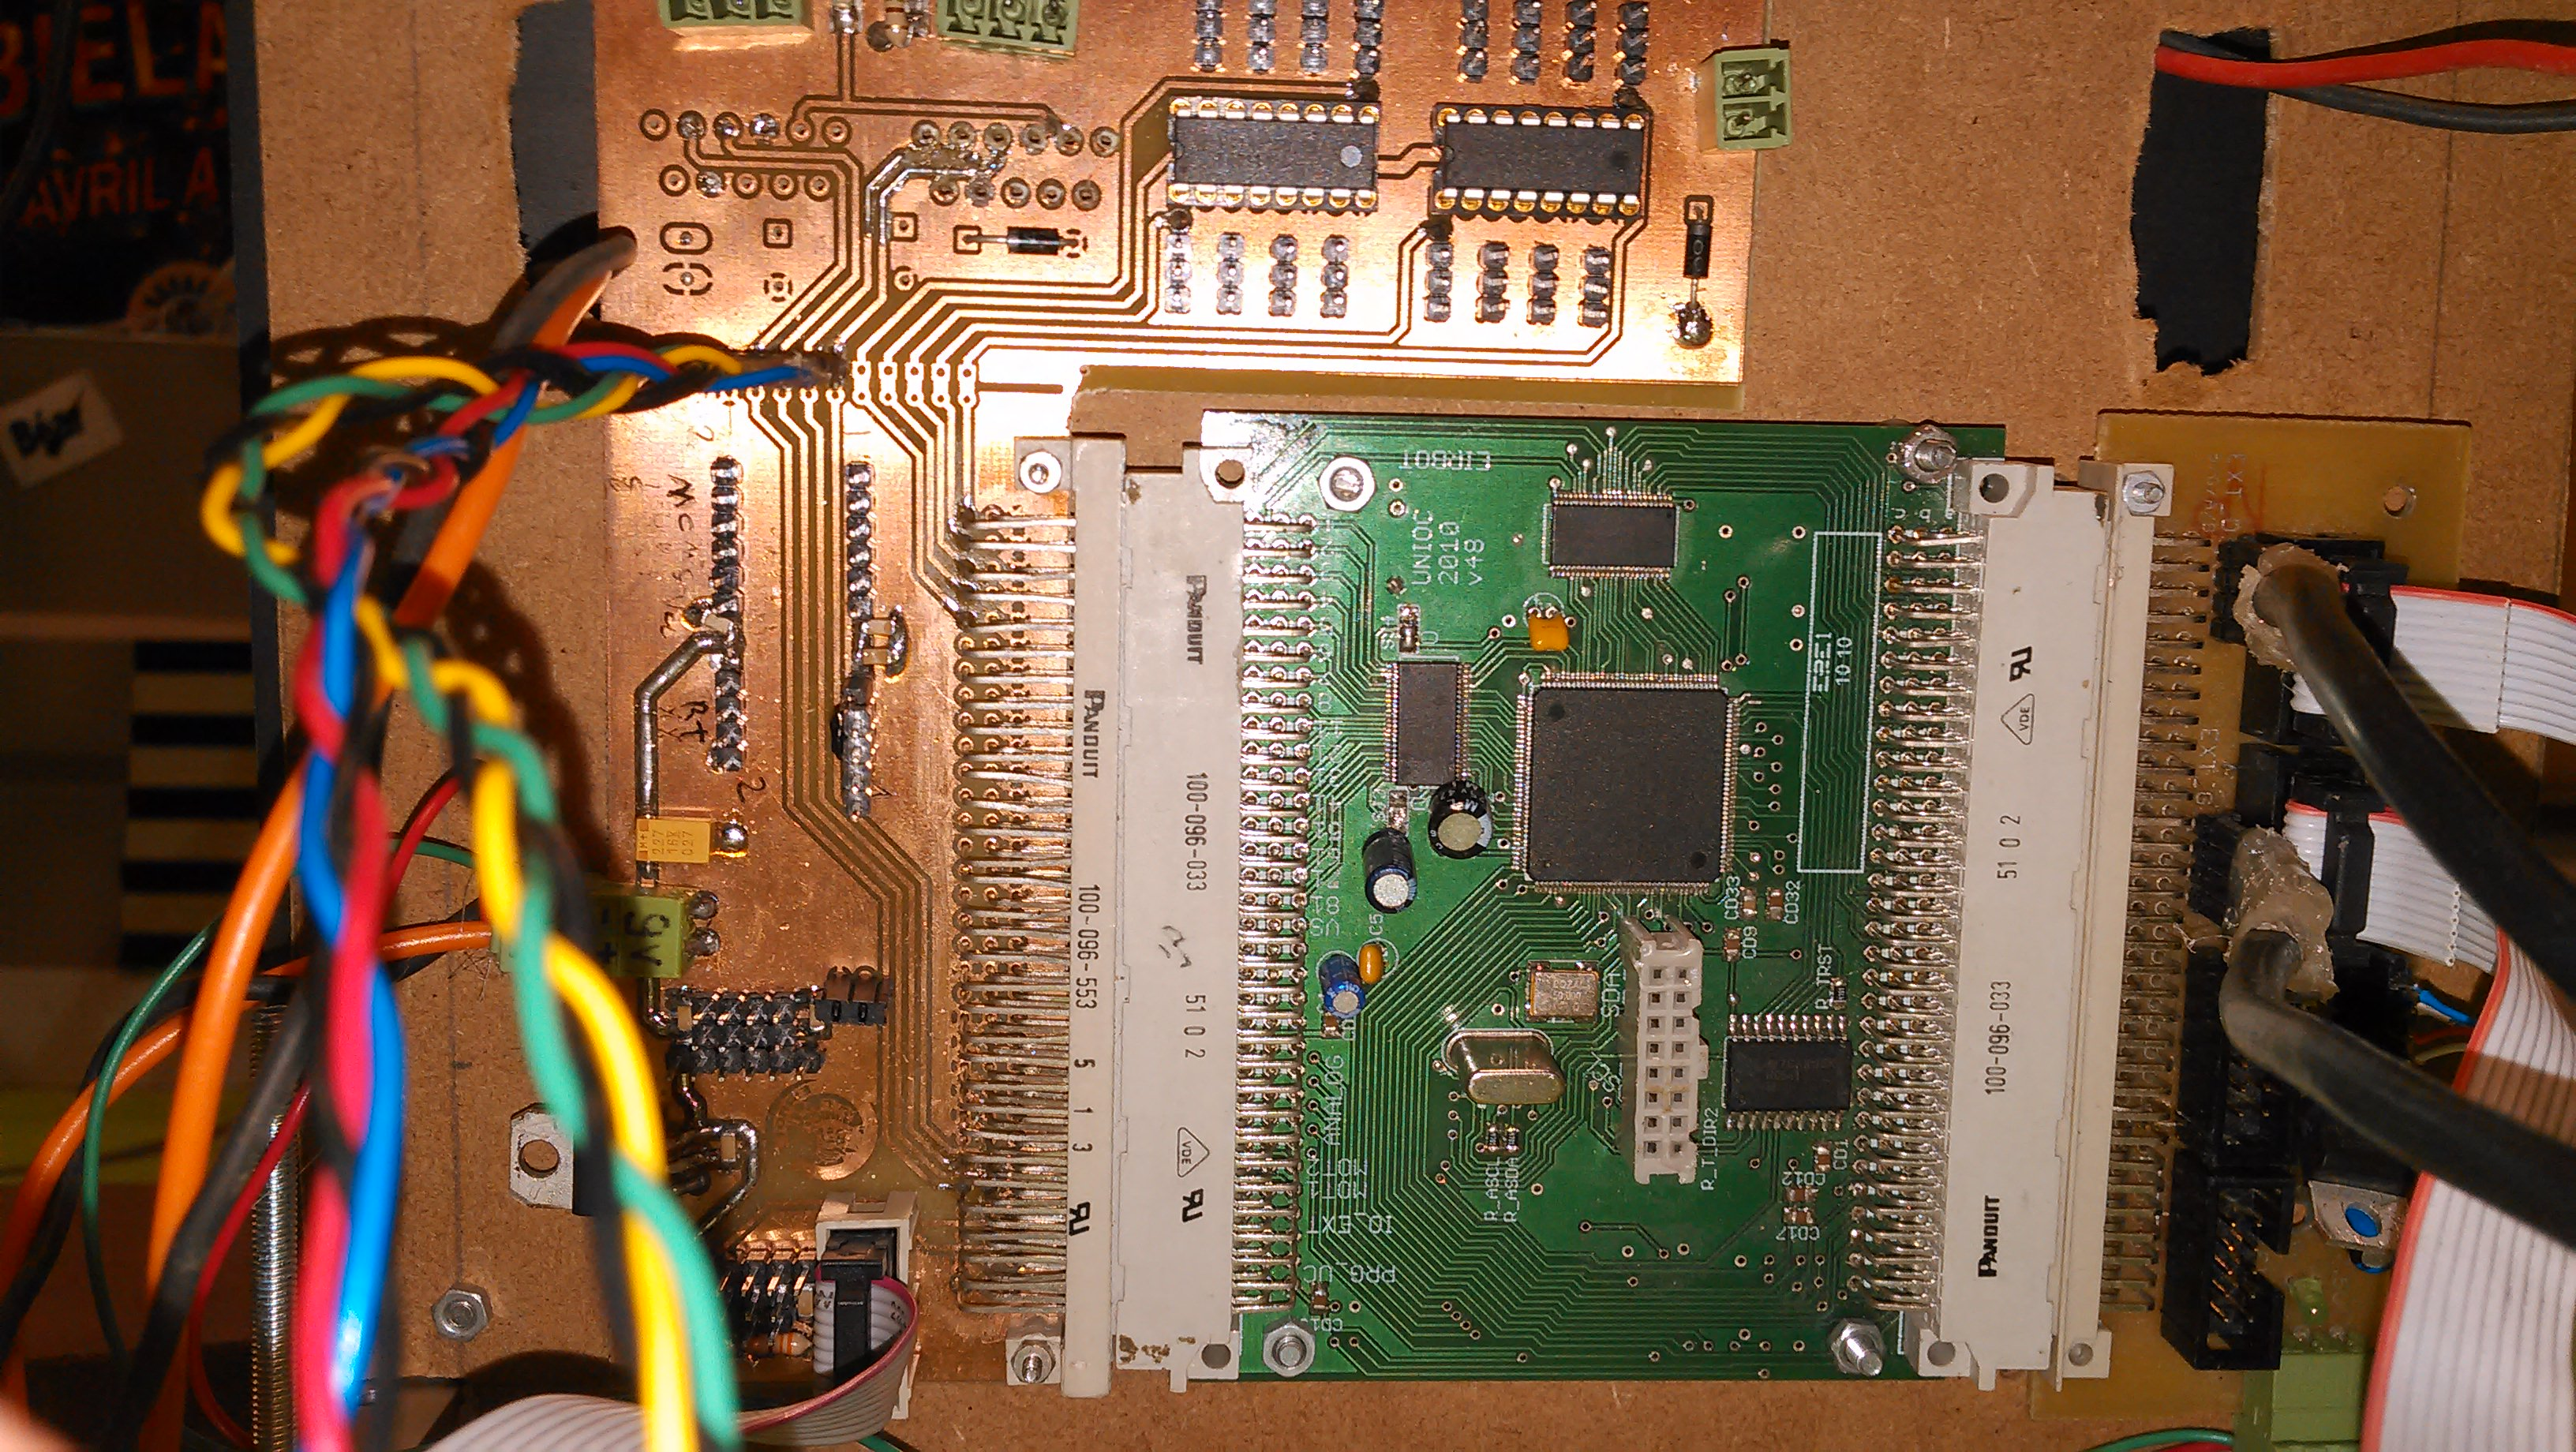
\includegraphics[scale=0.1]{unioc}
\caption{UNIOC : principale carte du robot.}
\label{unioc}
\end{figure}

\paragraph{}
La carte électronique principale du robot \ref{unioc} est appelée carte UNIOC. Cette carte contient toute la stratégie du robot, gère le déplacement, l'évitement d'éventuels adversaires. Elle dispose de l'essentiel de la puissance de calcul du robot. Jusqu'à présent, elle utilisait le framework Aversive, écrit par d'anciens élèves de l'école (expliqué ci-dessous). Cette carte envoie les commandes à tous les moteurs et actionneurs du robot. Elle communique également avec d'autres cartes telles que celle de détection d'adversaire \ref{rds} pour ajuster sa stratégie en fonction de la position des autres robots.

\begin{figure}[!h]
\centering
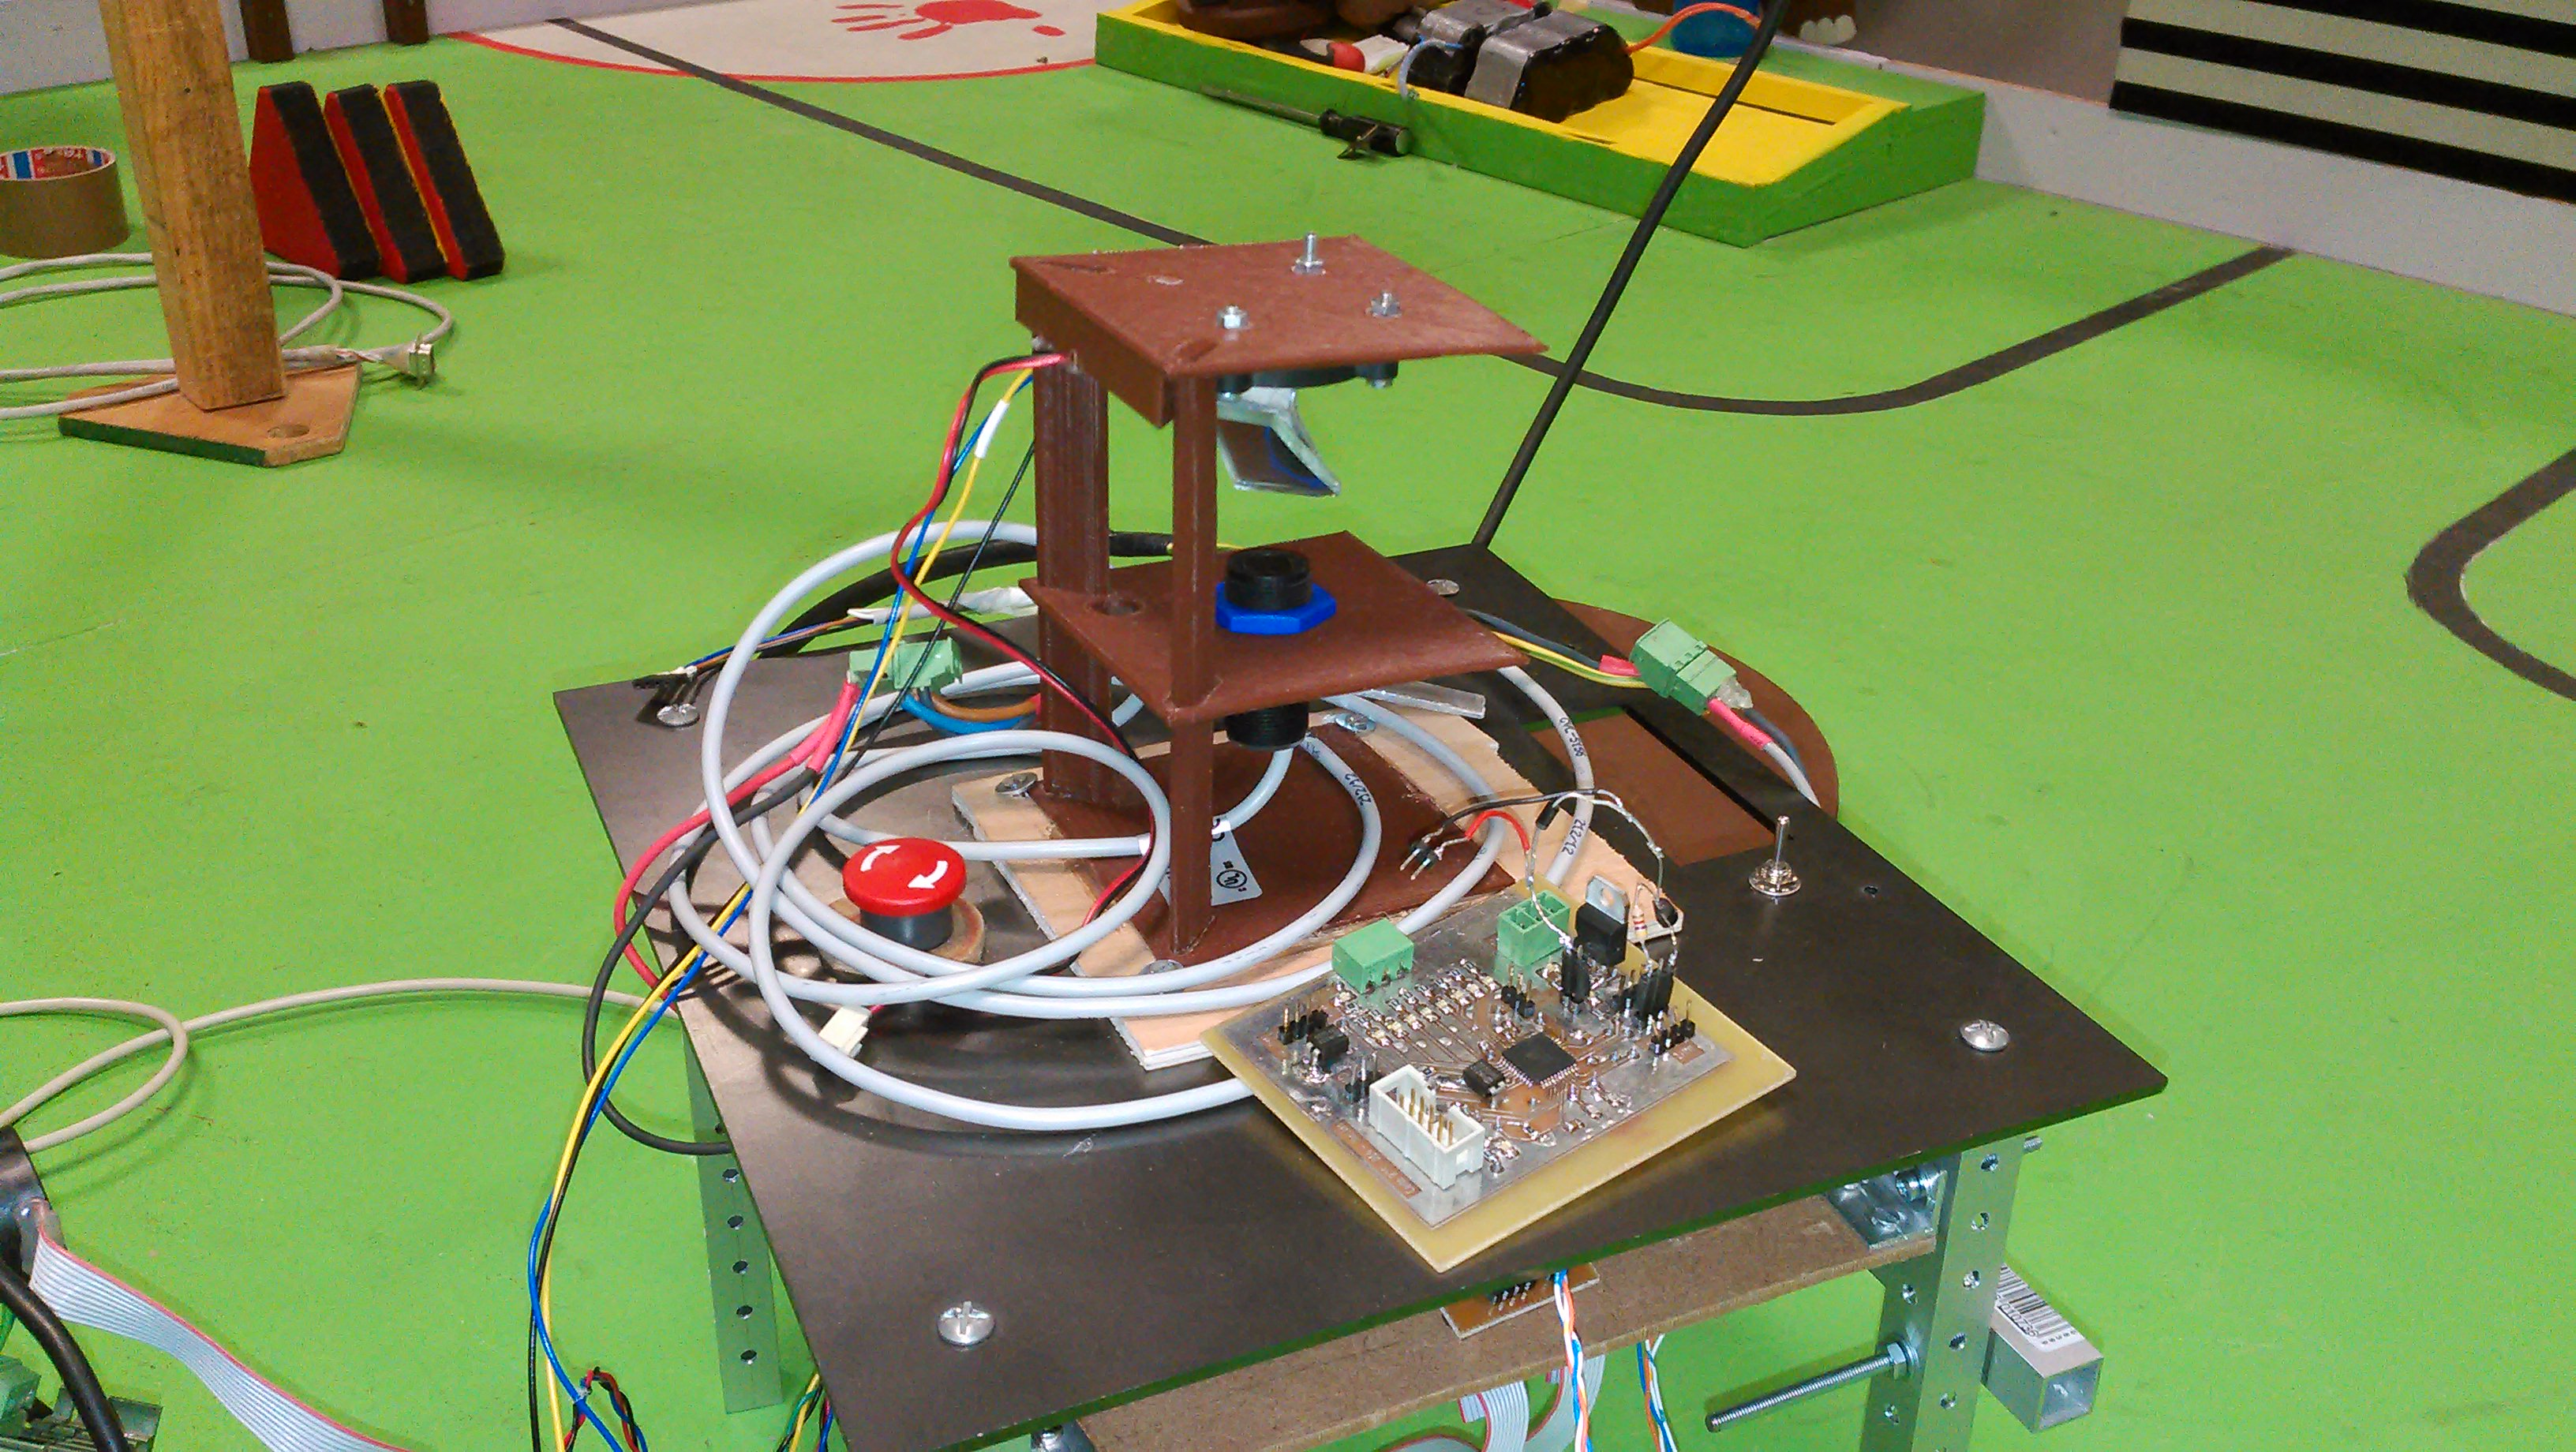
\includegraphics[scale=0.1]{rds}
\caption{Système de détection de robots adverses.}
\label{rds}
\end{figure}

\section{Objectifs}

Le résultat souhaité par le client EIRBOT est un simulateur de robot. Ce simulateur doit afficher le déplacement d'un ou plusieurs robot sur la table vue de dessus, en temps réel. Il prend en entrée un code robot et une description du robot et de la table. Un robot doit pouvoir interagir avec son environnement grâce à ses capteurs. Le simulateur doit donc être en mesure de calculer les valeurs à renvoyer aux capteurs du robot en fonction de s'il rencontre un obstacle, un autre robot, etc...

Cette spécification est primordiale pour le client, car le principal objectif du simulateur est d'afficher un déplacement du robot le plus proche possible de la réalité.
En effet, pour obtenir un bon score à la coupe de France de robotique à laquelle participe Eirbot, il est important de maîtriser son déplacement sur la table. Un déplacement "intelligent" comprend un évitement efficace des obstacles et des robots adverses, et il s'agit d'une des priorités pour l'équipe Eirbot.

\paragraph{}
Ce projet contient également, en partie, la réécriture du framework (Aversive) qui existe déjà à Eirbot et qui avait été écrit il y a 7 ans par des élèves de l'école. Ce framework gère les interruptions, propose des primitives de haut niveau pour déplacer le robot sur la table, et des interfaces de communication avec les entrées et sorties.

Le besoin de réécrire Aversive est dû au fait qu'au fil des ans, la compréhension de cet outil se perd et qu'il est de plus en plus difficile pour les nouvelles années de le débugguer ou de l'exploiter à son plein potentiel.
EIRBOT souhaite donc disposer d'un nouveau framework (Aversive++) mieux documenté. Cependant seule la réécriture de l'API d'Aversive++ est concernée par le projet SASIAE\footnote{Simulateur d'Asservissement de Stratégie et d'Intelligence Artificielle d'Eirbot}. 

Notre rôle a donc été la création de l'interface et le développement des fonctionnalités du nouveau framework destiné au simulateur, et l'association EIRBOT est en charge quant à elle de développer les mêmes fonctionnalités pour le microcontrôleur.

\paragraph{}
Le cahier des charges détaille les fonctionnalités souhaitées par EIRBOT pour le simulateur. De plus la majorité de l'équipe SASIAE étant également dans l'équipe Eirbot, ce qui n'aura pas été fait durant le PFA, notamment par manque de temps, sera implémenté plus tard par les membres d'Eirbot.

\paragraph{}
Le \textbf{S}imulateur d'\textbf{A}sservissement, de \textbf{S}tratégie et d'\textbf{I}ntelligence \textbf{A}rtificielle d'\textbf{E}IRBOT prenait ainsi vie, sous le nom plus élégant de SASIAE.

